%!TEX root = main.tex
\chapter{Multi-parameter Models}\label{ch:multiparam}

We have already met examples of multiple parameter estimation in the case of unknown uncertainty, where we have to estimate both the ``true'' value, $\mu$, and the uncertainty, $\sigma$.  In this chapter, we introduce the model of {\em linear regression}, which has multiple ``true'' value parameters and their uncertainty.  In the simple cases, we can calculate the estimates by hand and apply the same testing procedures as described in Chapter~\ref{ch:tests} (\emph{\nameref{ch:tests}} on page~\pageref{ch:tests}).  In the more complex cases we will have to rely on the computer to give us the estimates, but we can still interpret them in the same way as before.

\section{Simple Linear Regression}

In simple linear regression, we are given data consisting of two variables, typically denoted $x$ and $y$, where the value of one ($y$) depends on the other ($x$).  For example, consider the following data of heights ($x$) and shoe sizes ($y$) of a small number of individuals\cite{mclaren2012using} shown in Table~\ref{tbl:shoesize_subset} and Figure~\ref{fig:shoesize_subset}.  By eye we can see a direct correlation - the taller the person the larger shoe size.  

\begin{table}
\begin{center}
\begin{tabular}{cc}
Height [inches] & Shoe Size \\ \hline\hline
64.0 & 7\\
70.0 & 9\\
64.0 & 8\\
71.0 & 11\\
69.0 & 12\\
68.0 & 9\\
69.0 & 10\\
61.0 & 6\\
68.0 & 10\\
70.0 & 9
\end{tabular}
\end{center}
\label{tbl:shoesize_subset}
\caption{Heights (in inches) and shoe sizes from a subset of McLaren (2012) data.}
\end{table}

\begin{figure}
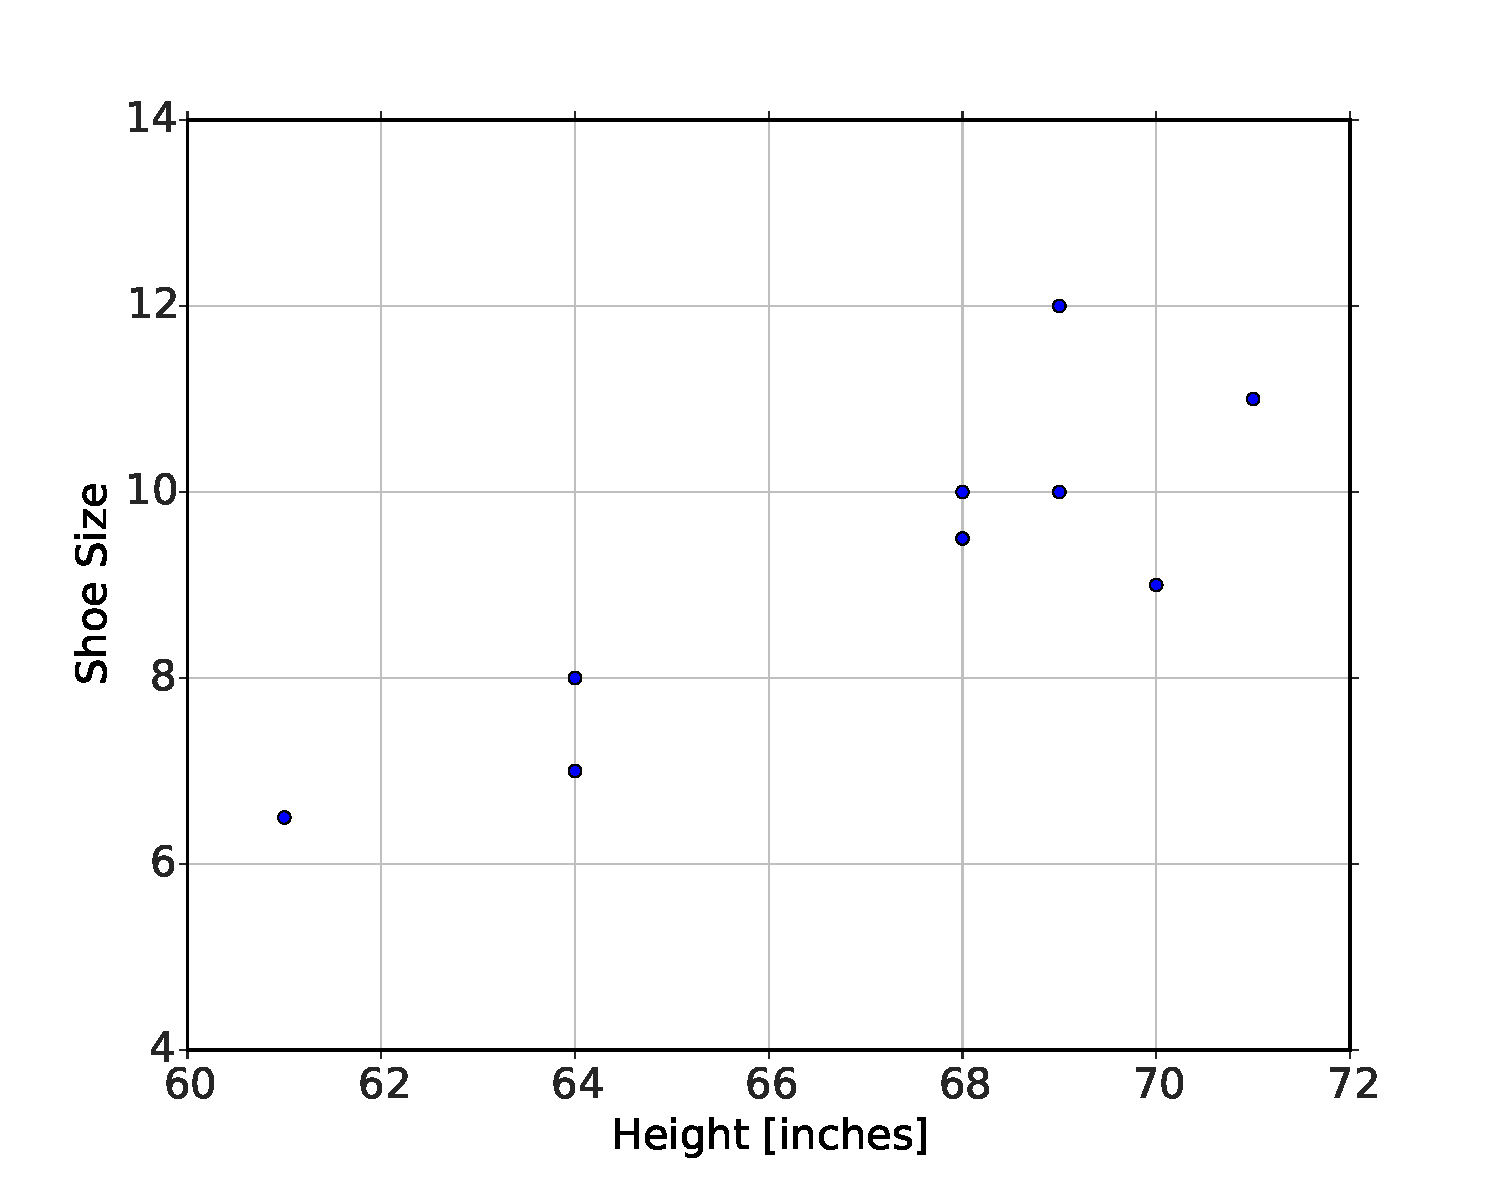
\includegraphics{shoesize_subset}
\label{fig:shoesize_subset}
\caption{Heights (in inches) and shoe sizes from a subset of McLaren (2012) data.}
\end{figure}

We propose a model of this data of the following {\em linear} form:
\beqn
y&=& m x + b
\eeqn
where $m$ is the slope and $b$ is the intercept.  Clearly this data doesn't form a perfect line, so there is some uncertainty in the slope, intercept, and predicted $y$ values.  We assume a Normal distribution for the uncertainties in the data, so the statistical model looks like, for each data point,
\beqn
y_{i}&=& m x_{i} + b + {\rm Normal}(0,\sigma)
\eeqn
where we want to obtain estimates,  $\hat{m}$ and $\hat{b}$, of the ``true'' values of the slope and intercept, respectively, as well as their uncertainties.  This is obtained by getting the posterior probability of the parameters,
\beqn
P(m,b|{\rm data})
\eeqn
Following our standard procedure,
\be
\i Specify the prior probabilities for the parameters being considered.  For most simple cases we begin with absolutely no knowledge of its value, and thus use a {\em uniform} prior probability for each parameter.
\i Write the top of Bayes' Rule, 
\beqn
P(m,b|{\rm data}) \sim \underbrace{P({\rm data}|m,b)}_{\mbox{\scriptsize Normal uncertainties}} \times \underbrace{P(m,b)}_{\mbox{\scriptsize uniform prior}}
\eeqn
\i Add up the values, and divide by this sum to get the final posterior probabilities.  This is done by the mathematicians, and we simply summarize the results here.
\ee
we obtain the posterior distributions for the parameters $m$ and $b$.  The calculations get too detailed to do by hand, but are very easy with the computer.  For the shoe size data in Table~\ref{tbl:shoesize_subset} we get the distributions shown in Figures~\ref{fig:shoesize_dist_slope} and ~\ref{fig:shoesize_dist_intercept} for the slope and intercept, respectively.  The most probable values then lead to the best fit, shown in Figure~\ref{fig:shoesize_fit}.

The Student-$t$ test clearly shows that the slope is non-zero (well over 95\% of the distribution lies to the right of zero), denoting a statistically significant effect on shoe size from height.  The magnitude of the slope, ${\rm slope}=0.42$, can be interpreted that every inch of height leads to a 0.42 increase in shoe size on average.


\begin{figure}
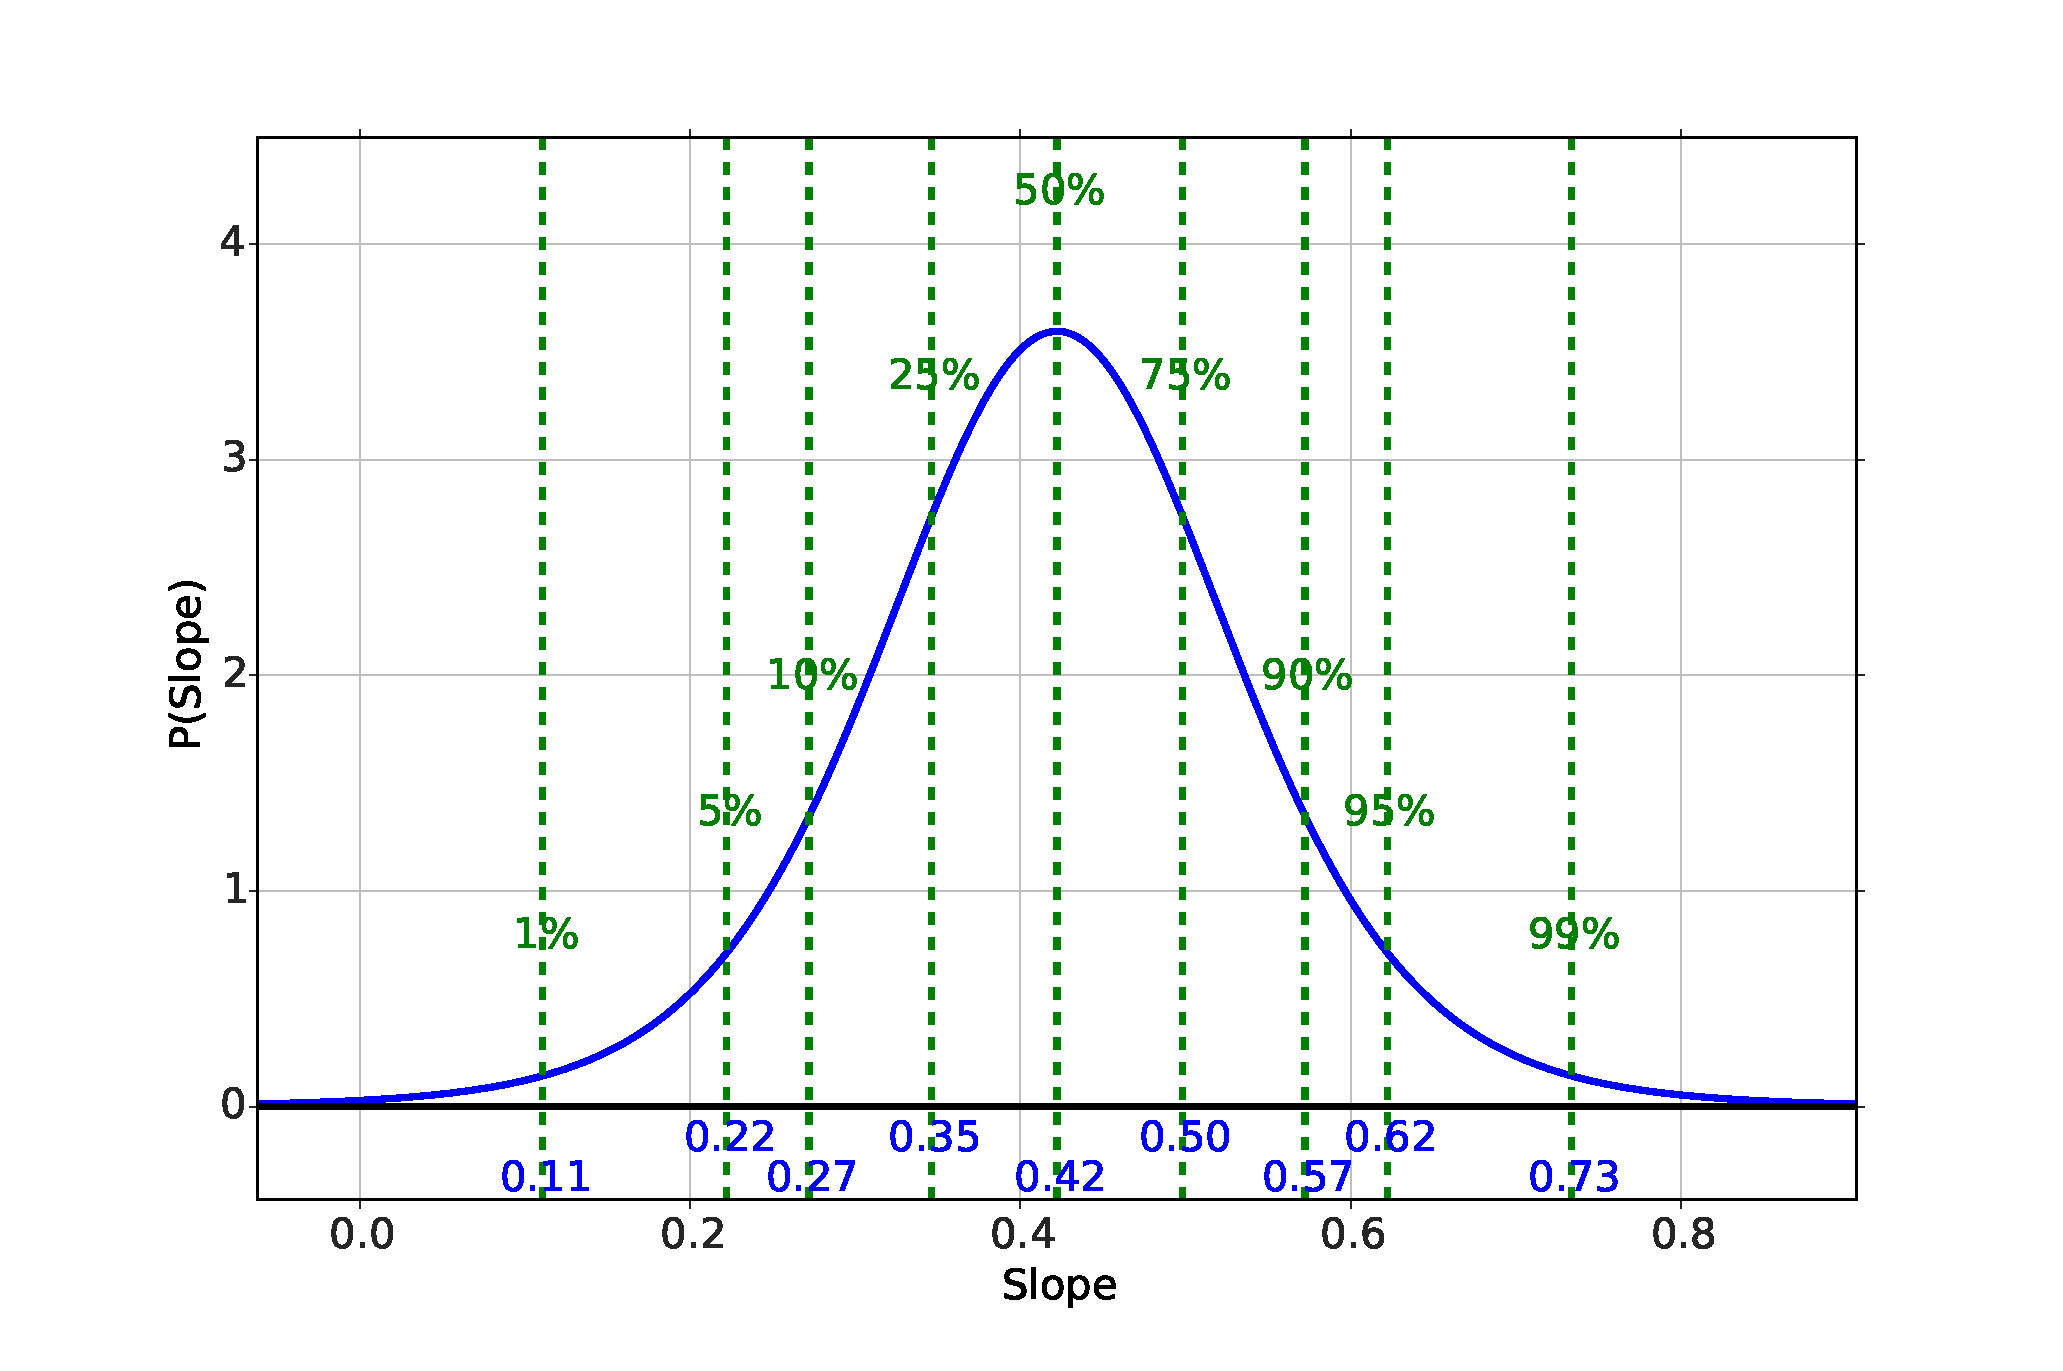
\includegraphics{shoesize_subset_slope}
\caption{Posterior distribution for the slope for the linear model on the shoe size data subset.}\label{fig:shoesize_dist_slope}
\end{figure}

\begin{figure}
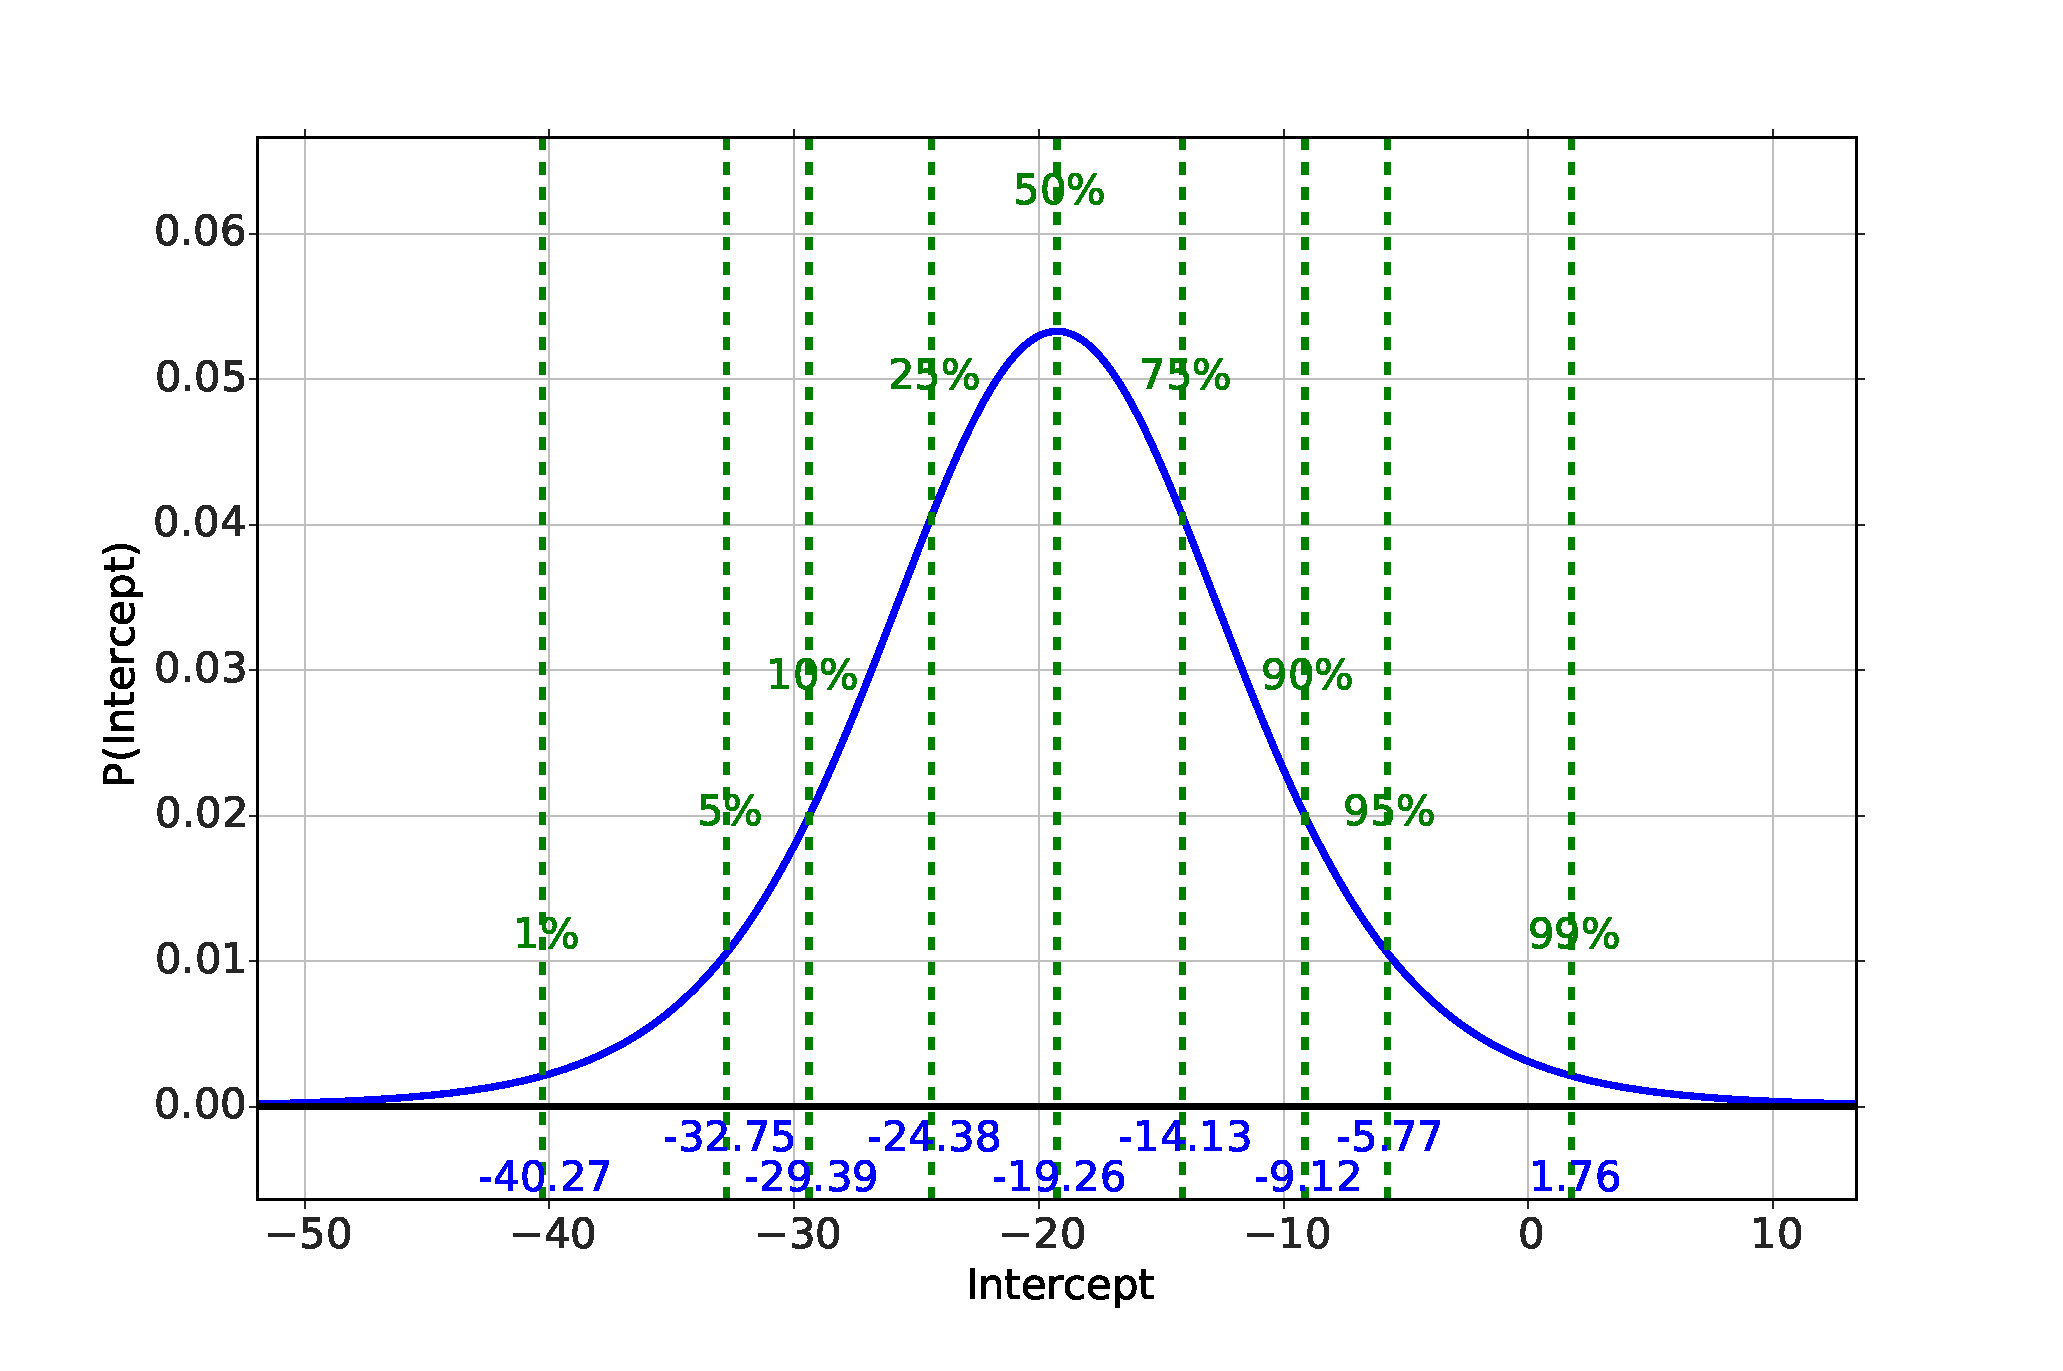
\includegraphics{shoesize_subset_intercept}
\caption{Posterior distribution for the intercept for the linear model on the shoe size data subset.}\label{fig:shoesize_dist_intercept}
\end{figure}

\begin{figure}
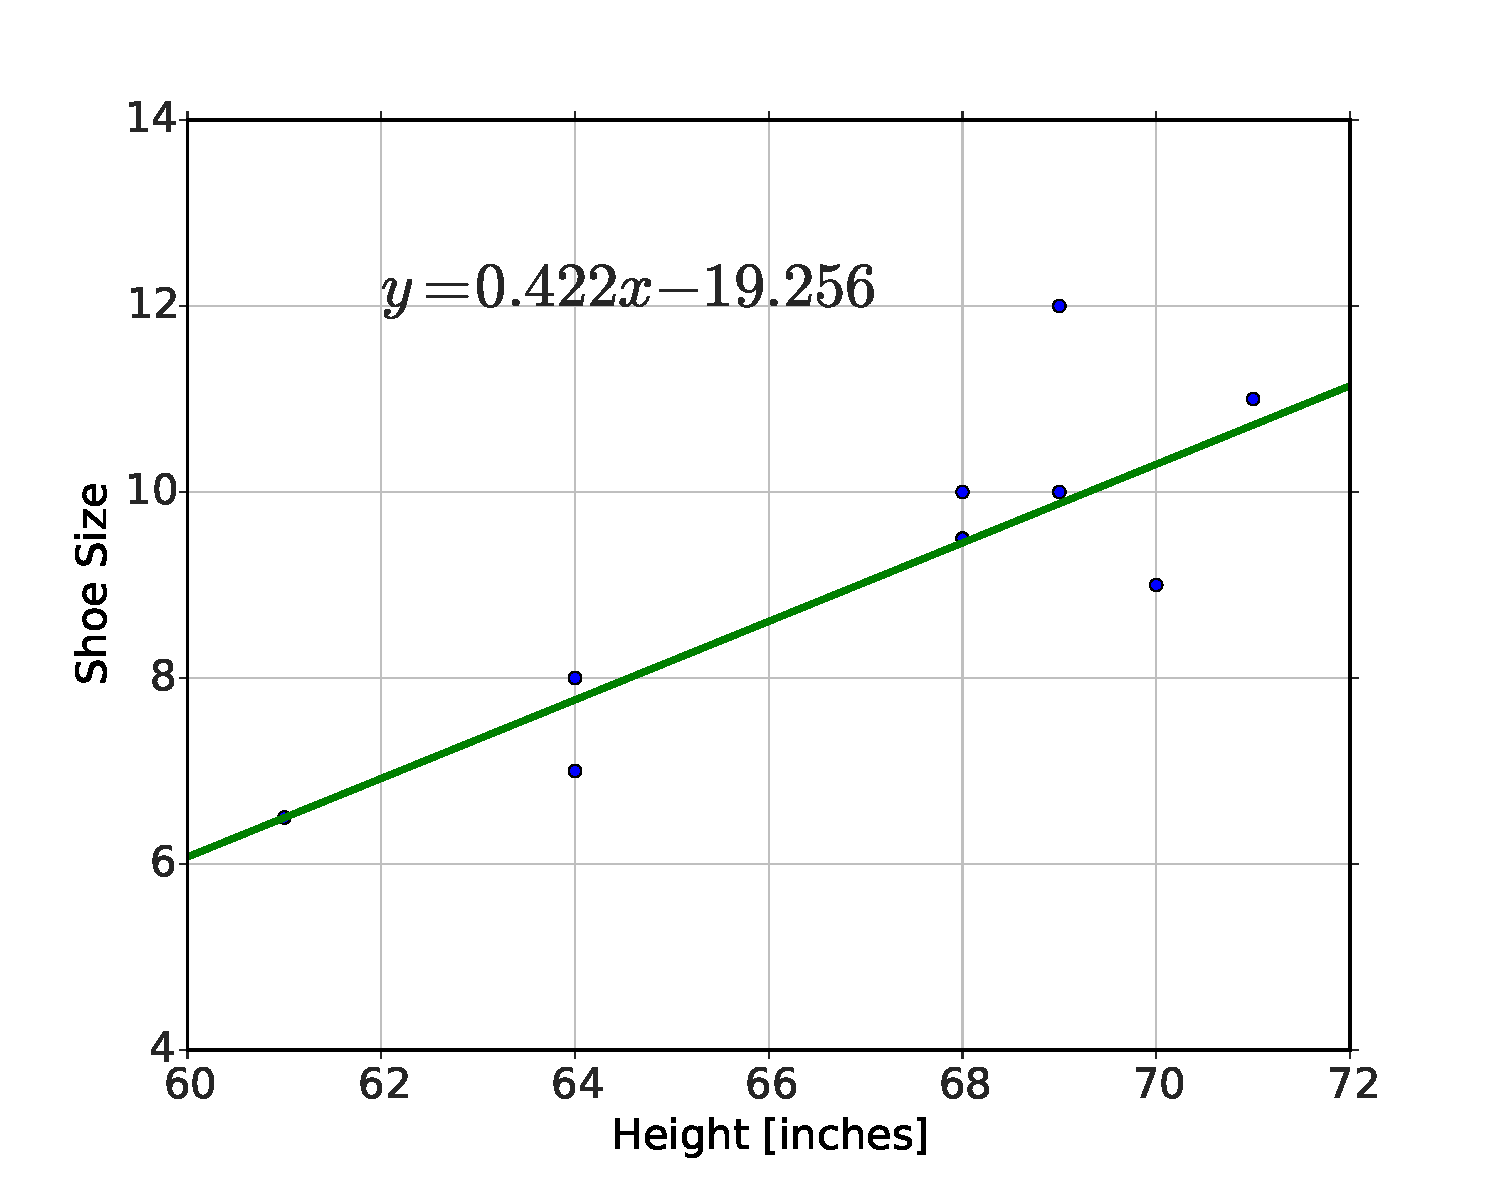
\includegraphics{shoesize_subset_fit}
\caption{Best linear fit for the shoe size data subset.}\label{fig:shoesize_fit}
\end{figure}


\subsection{Mean Squared Error}

Another way of looking at the same idea is to introduce the notion of \emph{Mean Squared Error} (MSE).  This is defined to be the number resulting from taking the predicted values minus the observed values, squaring them, and taking their mean.  The squaring ensures that deviations from the predictions both too high and too low are considered the same.  The closer the prediction overall, the smaller the resulting MSE.  Mathematically this is written as
\beqn
{\rm MSE} \equiv \frac{\sum_{i} \left(y_{i}- (\hat{m} x_{i}+\hat{b})\right)^{2}}{N}
\eeqn
One can intuitively think of getting the best fit as adjusting the slopes and intercepts, calculating the MSE for each, and stopping when you reach a minimum value.  An example of this is shown in Figure~\ref{fig:shoesize_mse}.

\begin{figure}
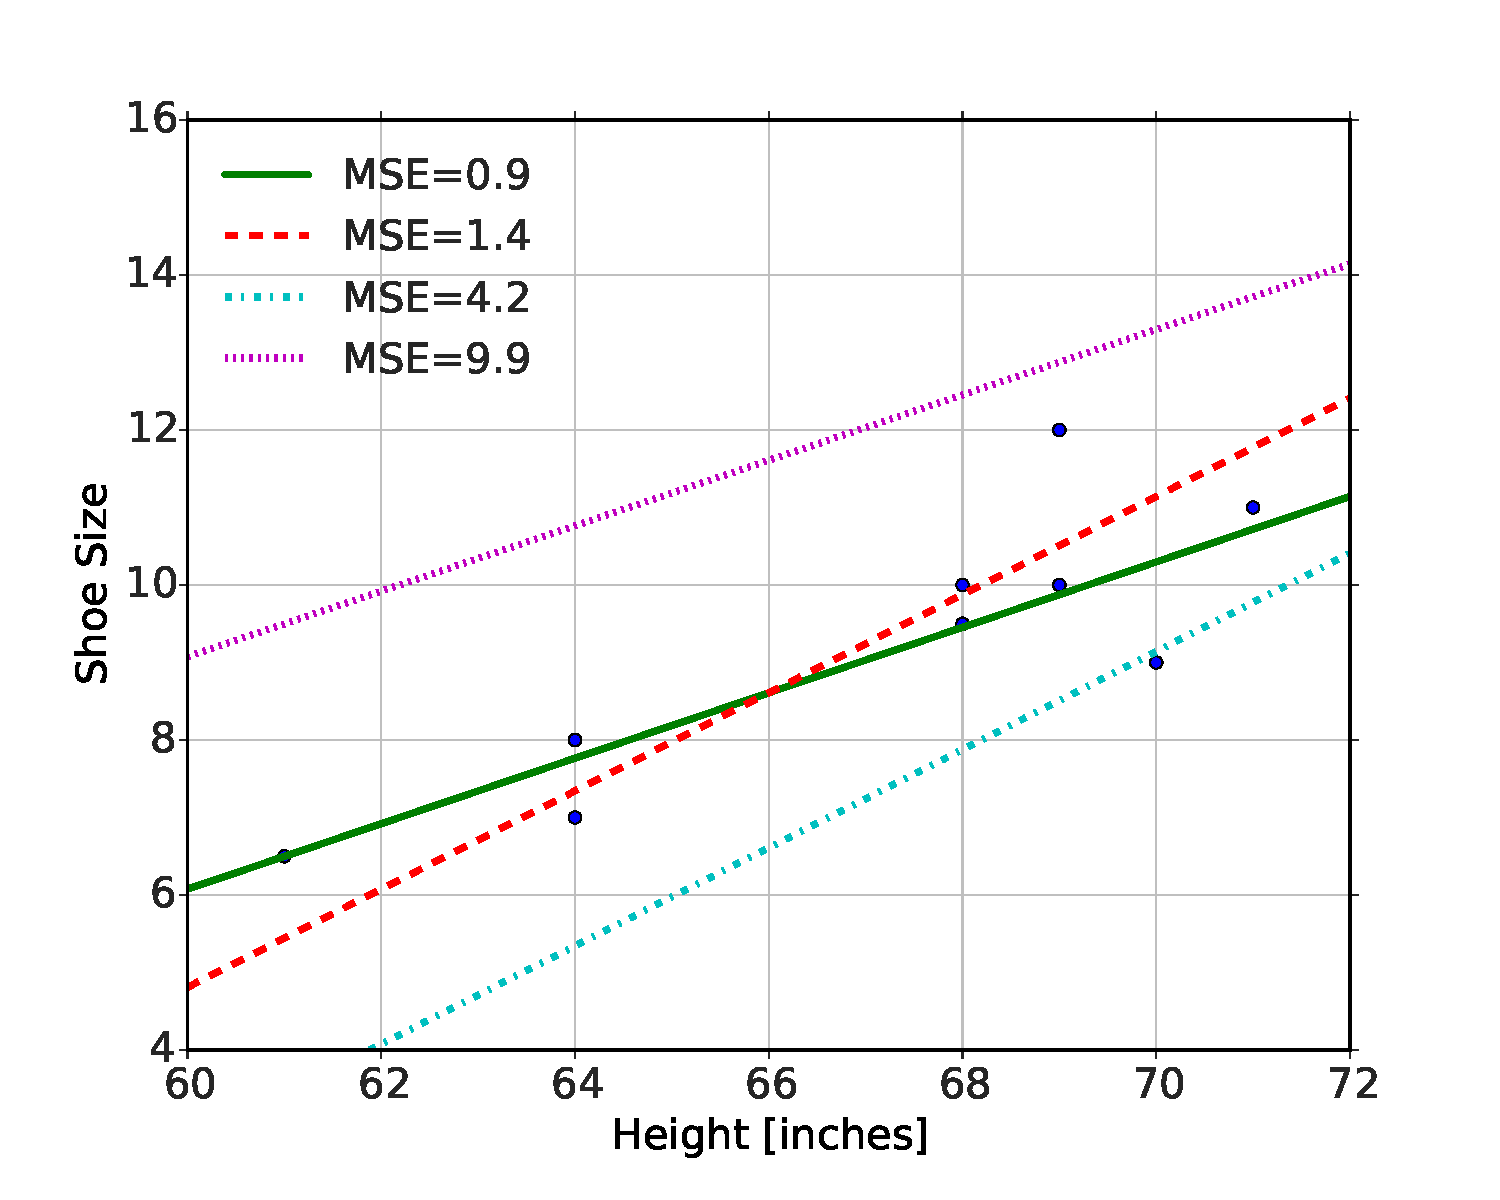
\includegraphics{shoesize_subset_regression_mse}
\caption{Minimizing the Mean Squared Error (MSE) results in the best linear fit for the shoe size data subset.}\label{fig:shoesize_mse}
\end{figure}


\subsection{An Educational Example}

The following example is from a data set on school expenditures and SAT scores.\cite{guber1999getting}  We plot the total SAT scores as a function of expenditures, perform a linear model fit, and present the best values and their uncertainties in Figure~\ref{fig:sat}.  The model is

\beqn
{\rm total} &=& {\rm intercept} + {\rm slope}\cdot{\rm expenditure}
\eeqn

\begin{figure*}
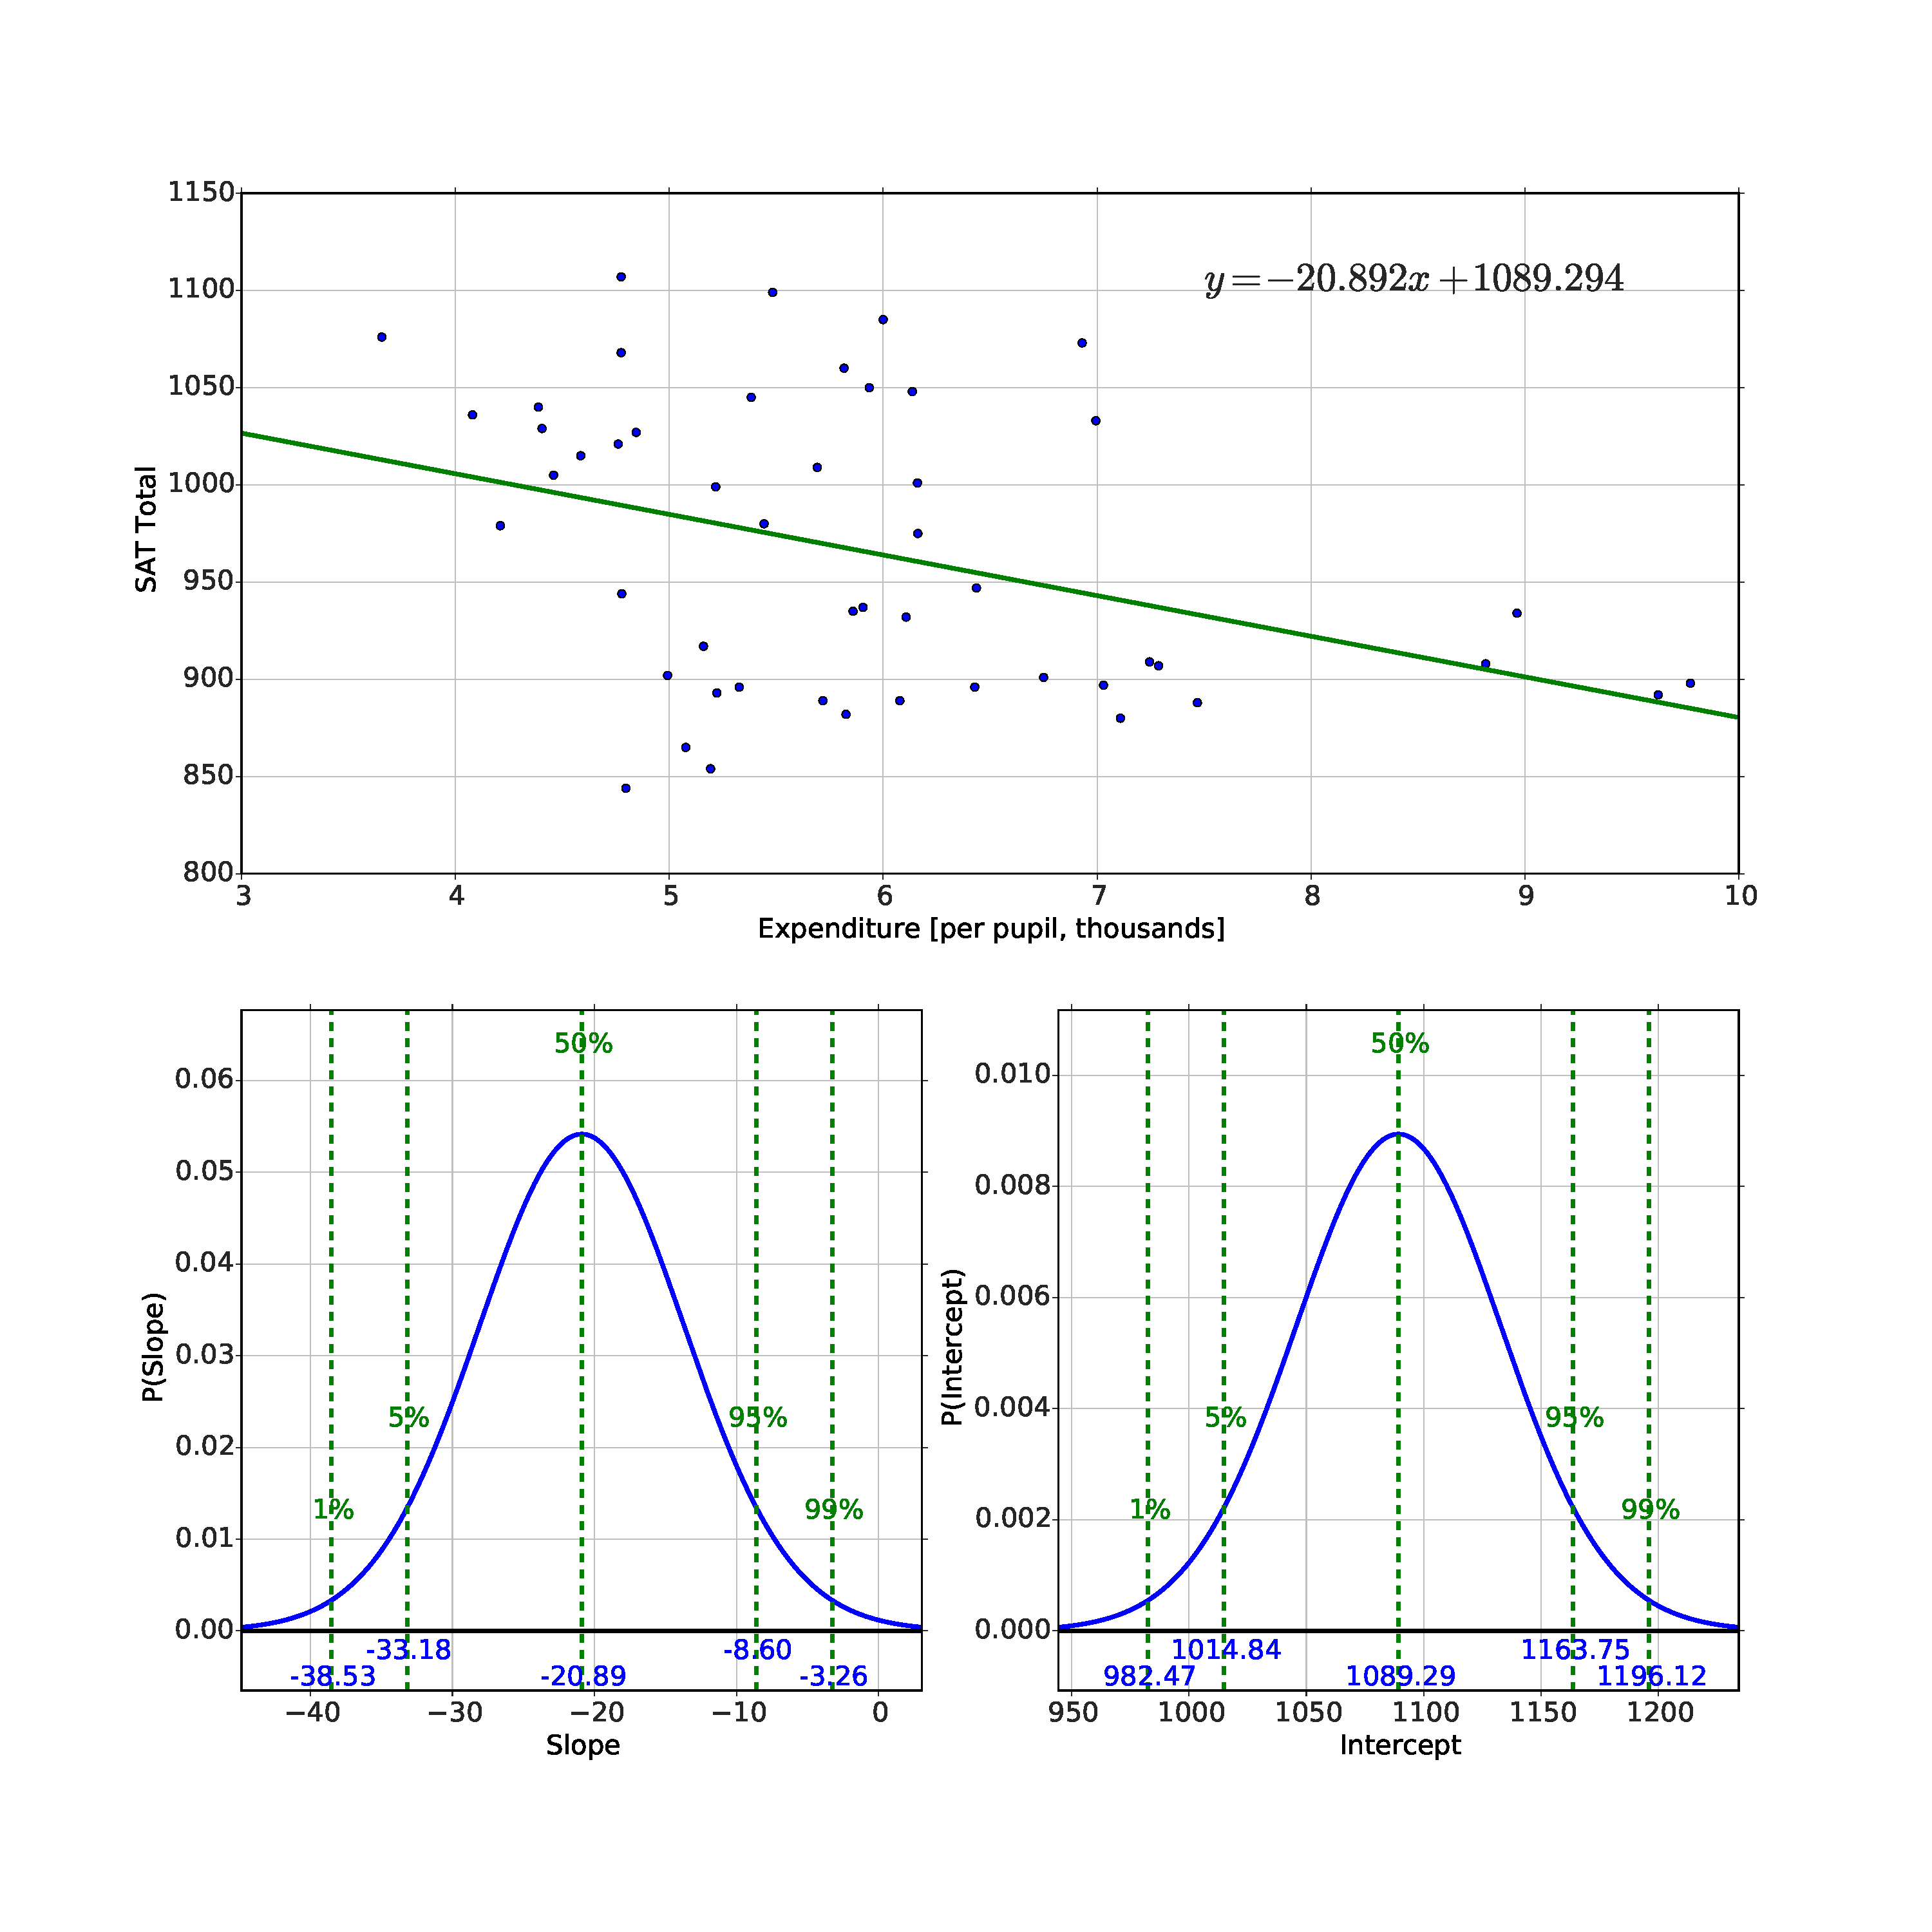
\includegraphics{sat_result}
\caption{Total SAT score vs expenditure (top) and the distributions for the slope (bottom left) and intercept (bottom right).}\label{fig:sat}
\end{figure*}

What is immediately odd is that this result seems to suggest the following:

\be
\i The \emph{larger} the expenditure per pupil the \emph{lower} the SAT scores.
\i For each thousand dollars spent per pupil, the total SAT score goes down 20 points.
\i If you spent zero dollars per pupil, you'd reach a maximum of SAT score of 1089.
\ee

This seems counter intuitive to say the least.  What is going on here? \marginnote{This is perhaps the most important lesson of regression.  When you see an effect, make sure to think of any variables that might also be effected that may give rise to the illusion of an effect.  It is critical that one get in this habit, or you will be at the whim of every unscrupulous statistician.}  What is happening is that there are other variables that are related to the expenditure which then lead to lower SAT scores on average.  Such a \emph{confounding} variable needs to be taken into account in what is called \emph{controlling} for a variable.

For example, if we look at the relationship between expenditure per pupil and the percent of students taking the SAT we see a pattern, shown in Figure~\ref{fig:percent_taking}.  The more that is spent per pupil, the more students - both bad and good - take the SAT.  Thus, even if expenditure helps students, the fact that the percentage of students taking the exam increases creates the illusion of the opposite. The next section states how you can overcome this problem.


\begin{figure*}
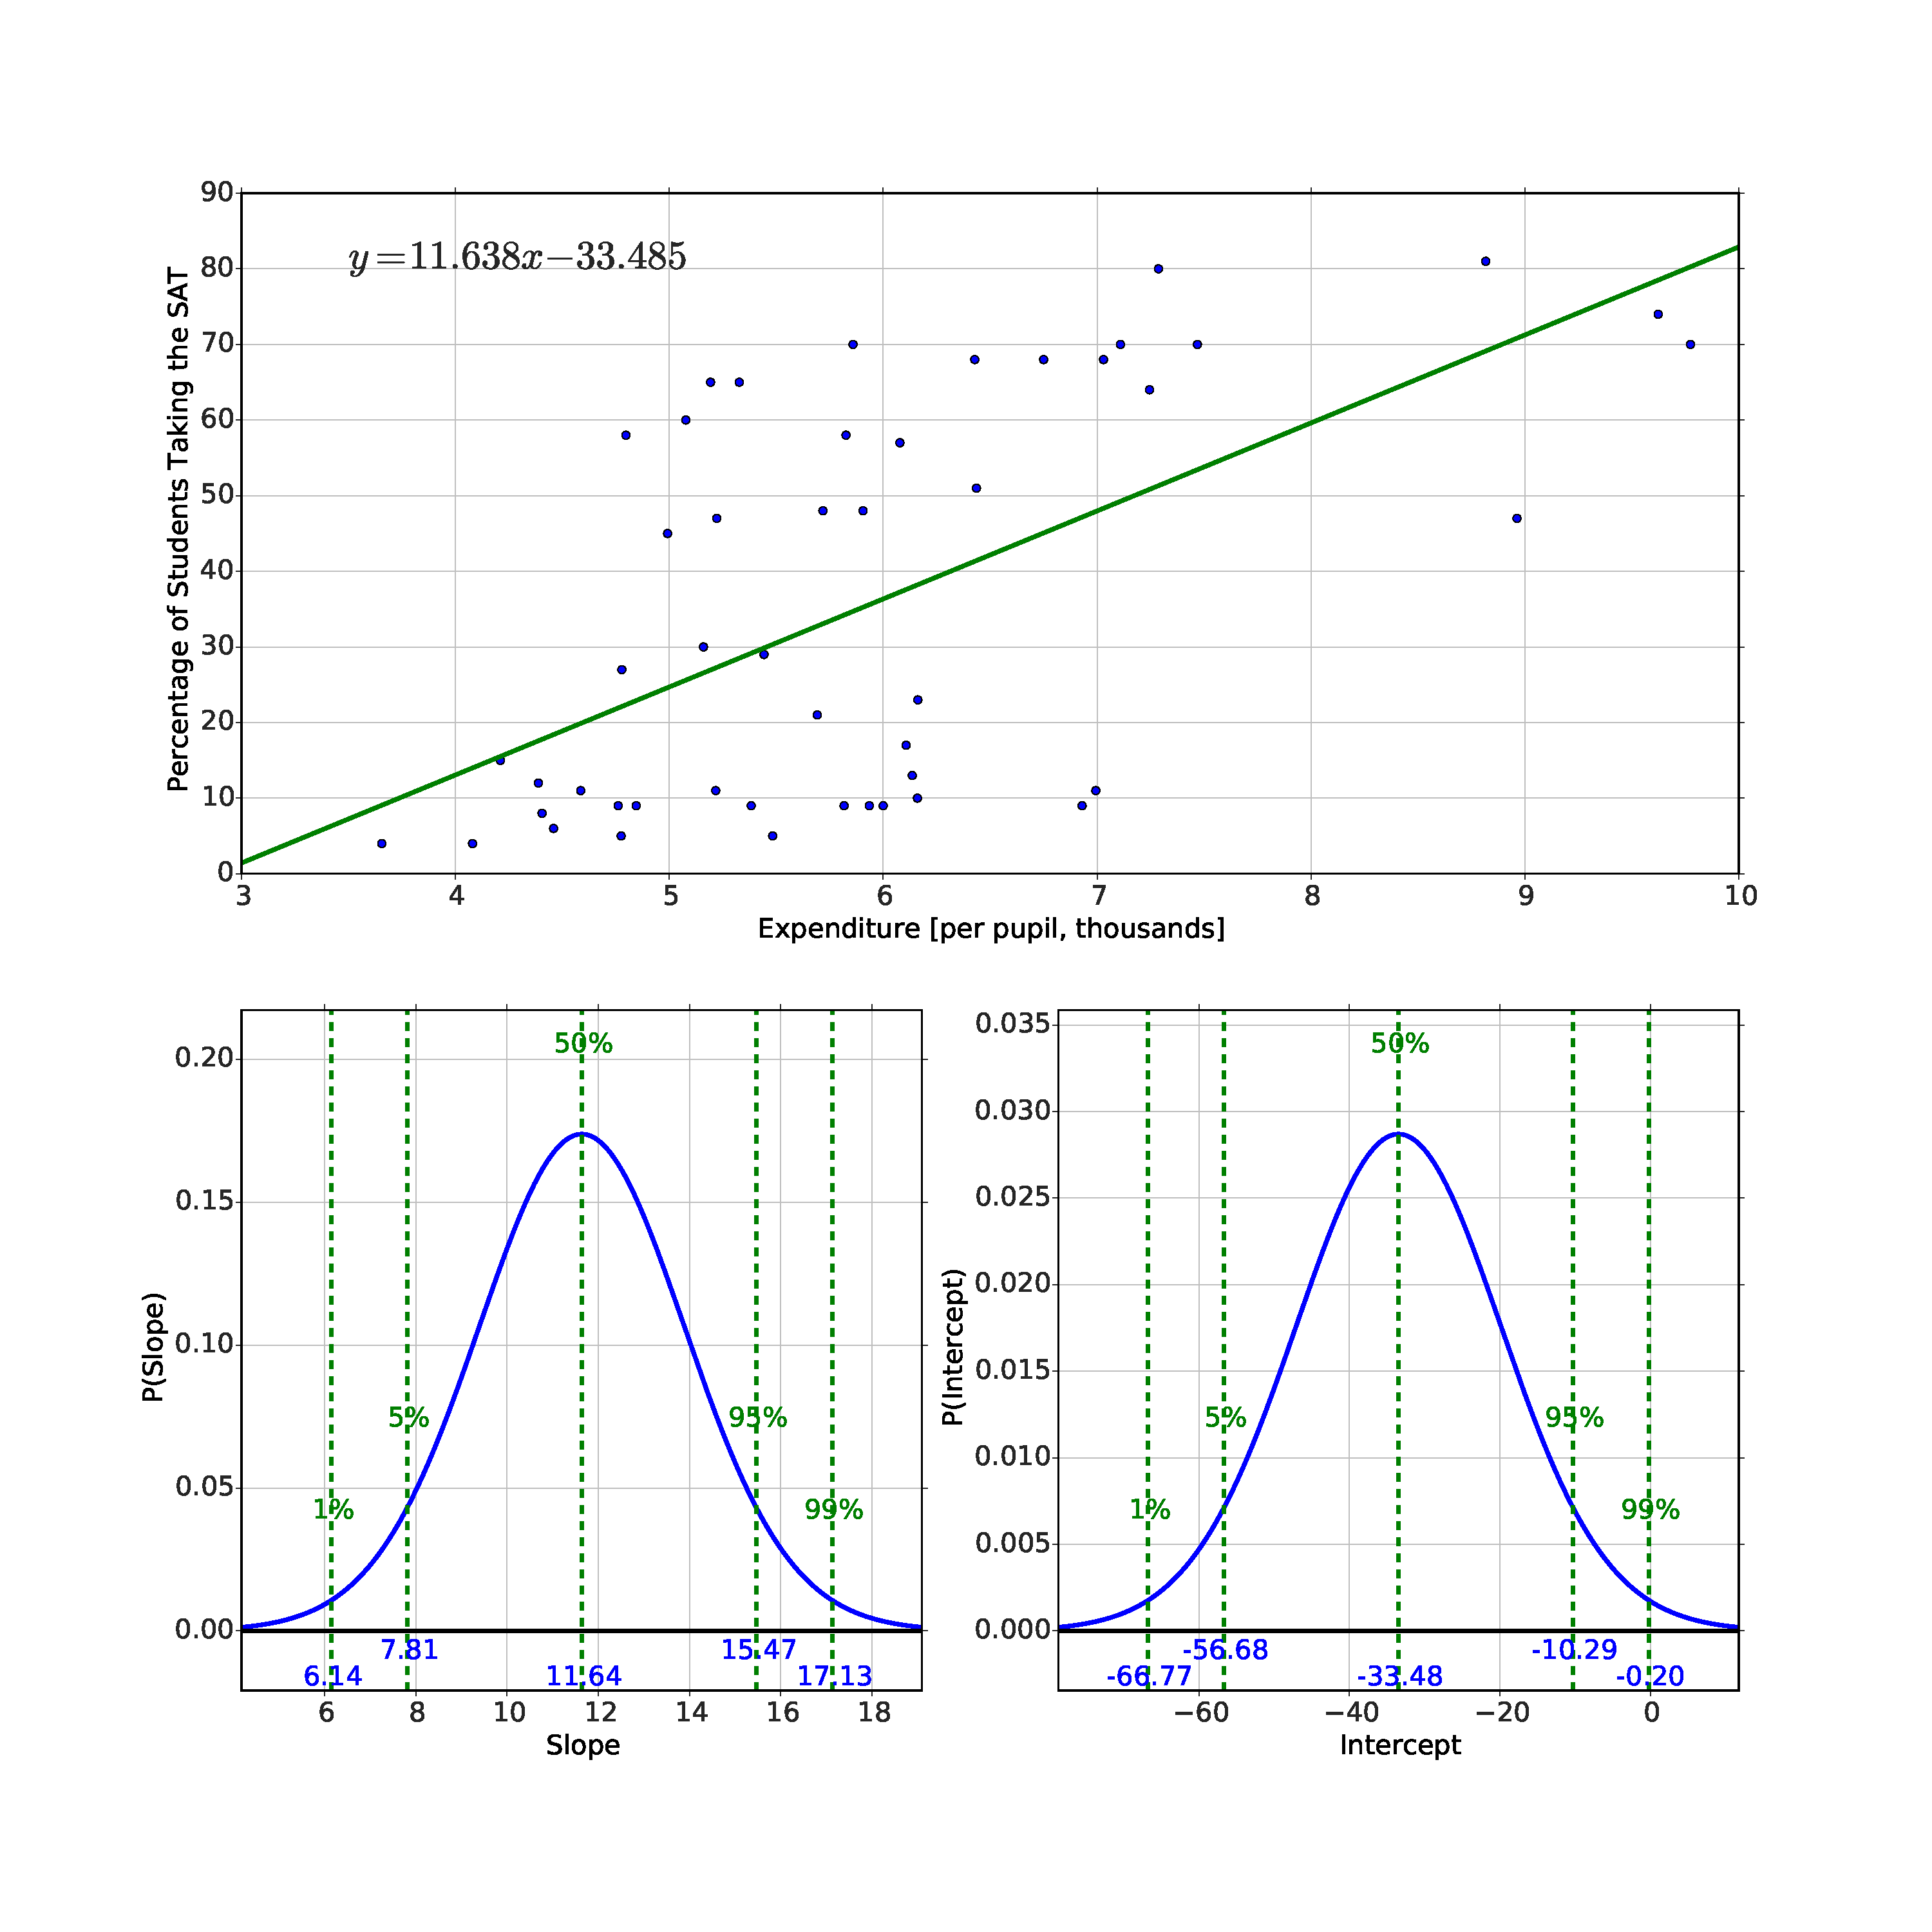
\includegraphics{sat_result_percent_taking}
\caption{Percent of students taking the SAT vs per pupil expenditure (top) and the distributions for the slope (bottom left) and intercept (bottom right).}\label{fig:percent_taking}
\end{figure*}


\section{Multiple regression}

In order to control for a variable that may be affecting our result, we simply expand our linear model, including slopes (also called \emph{coefficients}) for each of the different variables.  Once we do this, visualization becomes challenging because we move into three or more dimensions.   Instead of $m$ for the slope, the multiple slopes are typically labeled with the greek letter $\beta$ and numbered, such as $\beta_{1}, \beta_{2},$ etc...  The intercept is then labeled $\beta_{0}$.  The model structure, however, is the same, and can be written
\beqn
y=\beta_{0}+ \beta_{1}x_{1}+\beta_{2}x_{2} \cdots
\eeqn
where the different $x_{1}$, $x_{2}$, etc... denote different variables.  For the example of the SAT scores, we might have

\beqn
{\rm total} &=& \beta_{0} + \beta_{1}\cdot{\rm expenditure} + \beta_{2}\cdot{\rm percent\_taking}
\eeqn
where $\rm percent\_taking$ is a variable representing the percent of students taking the exam.  Including this variable gives the posterior distributions shown in Figure~\ref{fig:sat_multiple}.  Notice that the effect of expenditure is both statistically significant and \emph{positive}.  We can interpret the values in the following way.
\bi
\i For each \$1000 more spent per pupil the total SAT score increases on average by 12.29.
\i For each percent increase in students taking the SAT, the total SAT score \emph{decreases} on average by 2.29.
\ei

Have we controlled for all of the effects?  Perhaps not!  This is where the ingenuity and expertise of the person analyzing the problem comes into play.


\begin{figure}
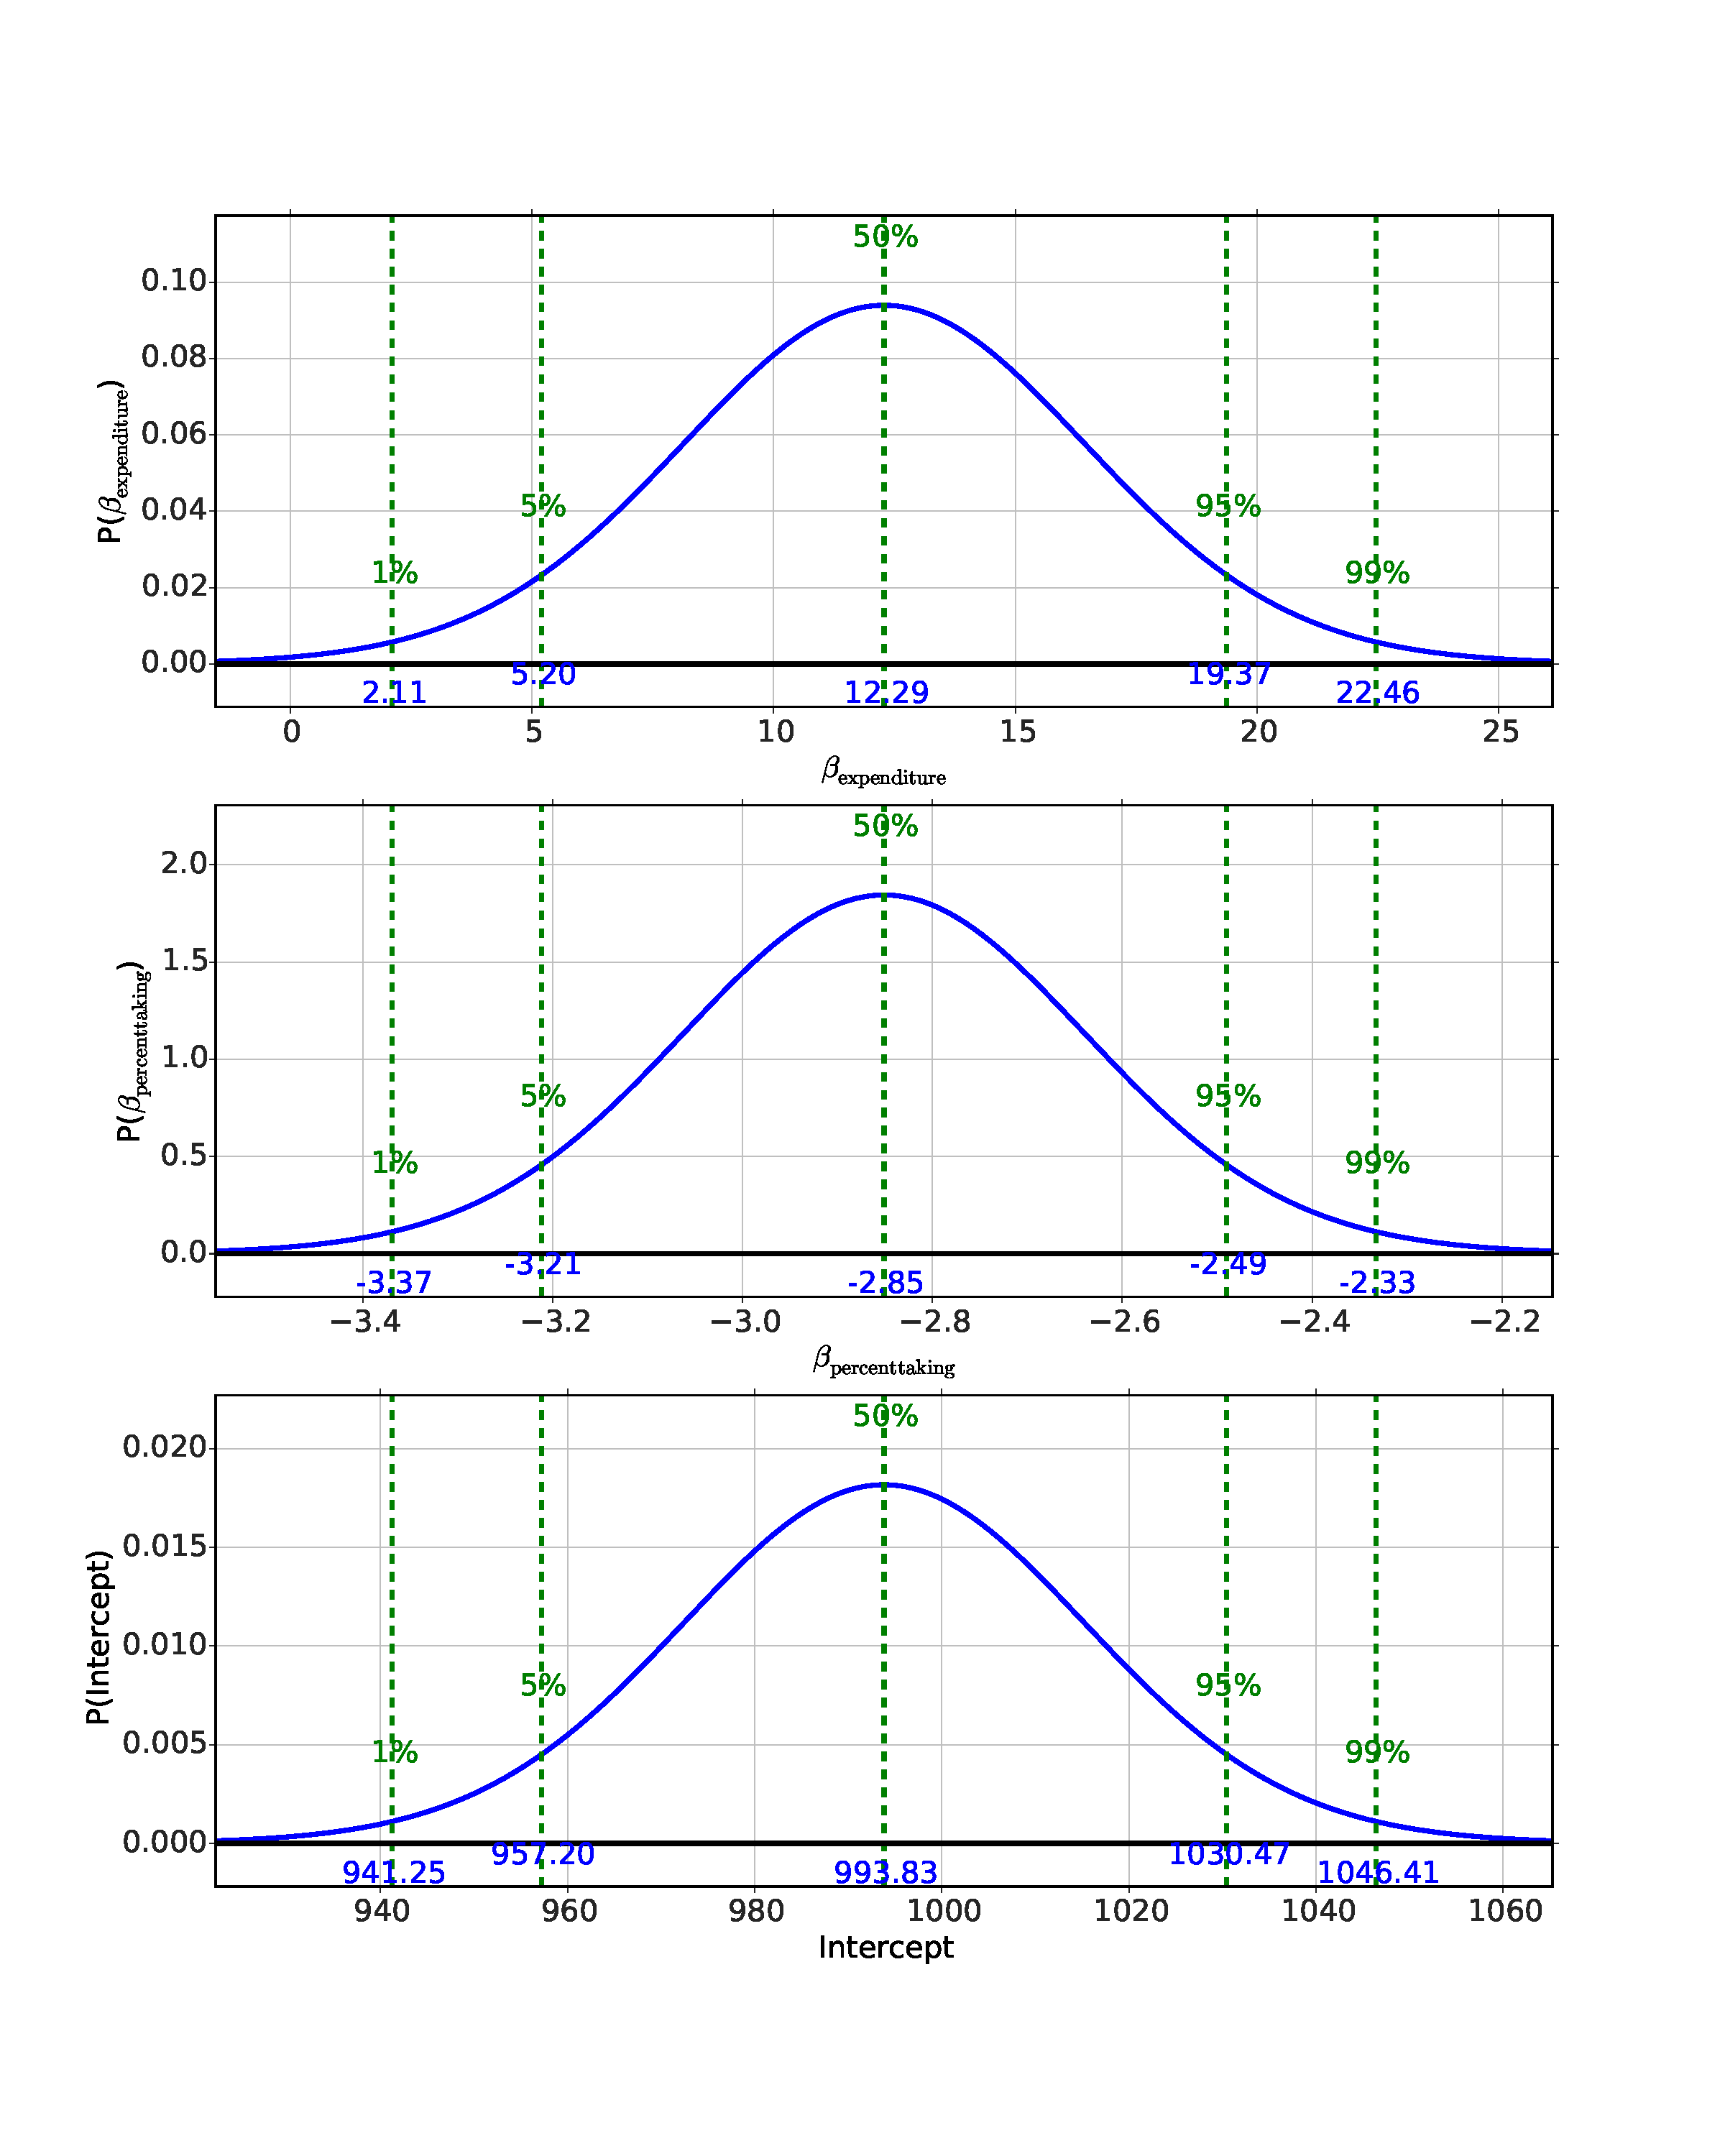
\includegraphics{sat_multiple}
\caption{The posterior distributions for coefficients on the expenditure term, the percent taking term, and the intercept.}\label{fig:sat_multiple}
\end{figure}



\section{Computer Examples}
\begin{fullwidth}
\begin{lstlisting}
from sie import *
\end{lstlisting}

\begin{lstlisting}
data=load_data('data/shoesize.xls')
\end{lstlisting}

\begin{lstlisting}
data.head()
\end{lstlisting}

\begin{verbatim}
   Index Gender  Size  Height
0      1      F   5.5      60
1      2      F   6.0      60
2      3      F   7.0      60
3      4      F   8.0      60
4      5      F   8.0      60
\end{verbatim}

\begin{lstlisting}
import random
\end{lstlisting}

\begin{lstlisting}
random.seed(102)
rows = random.sample(data.index, 10)
newdata=data.ix[rows]
data=newdata
data
\end{lstlisting}

\begin{verbatim}
     Index Gender  Size  Height
60      61      F   7.0      64
251    252      M   9.0      70
69      70      F   8.0      64
290    291      M  11.0      71
247    248      M  12.0      69
156    157      F   9.5      68
231    232      M  10.0      69
17      18      F   6.5      61
216    217      M  10.0      68
252    253      M   9.0      70
\end{verbatim}

\begin{lstlisting}
plot(data['Height'],data['Size'],'o')
gca().set_xlim([60,72])
gca().set_ylim([4,14])
xlabel('Height [inches]')
ylabel('Shoe Size')
\end{lstlisting}

\begin{verbatim}
<matplotlib.text.Text at 0x10adae0d0>
\end{verbatim}

\begin{center}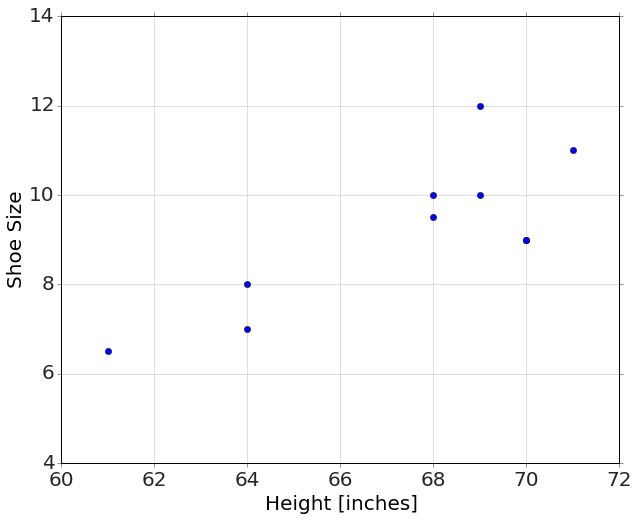
\includegraphics[width=4.5in]{Regression/Regression_fig0.png}\end{center}

\begin{lstlisting}
result=regression('Size ~ Height',data)
\end{lstlisting}

\begin{verbatim}
<matplotlib.figure.Figure at 0x10d200710>\end{verbatim}

\begin{center}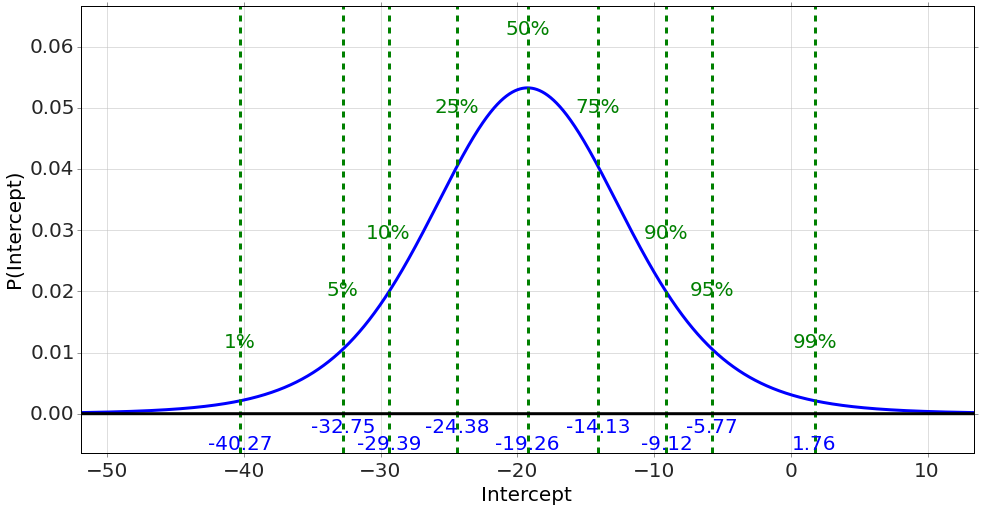
\includegraphics[width=4.5in]{Regression/Regression_fig1.png}\end{center}

\begin{verbatim}
<matplotlib.figure.Figure at 0x10d702610>\end{verbatim}

\begin{center}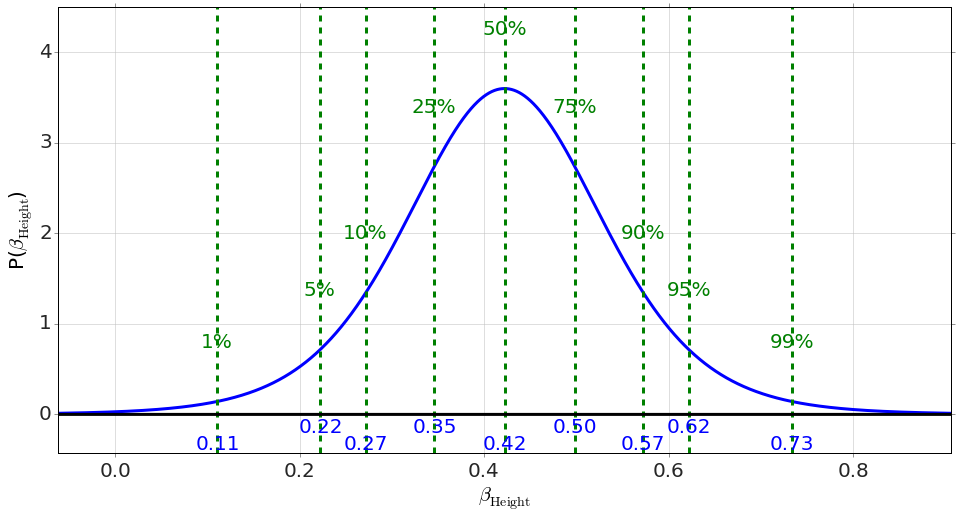
\includegraphics[width=4.5in]{Regression/Regression_fig2.png}\end{center}

\begin{lstlisting}
plot(data['Height'],data['Size'],'o')

h=linspace(60,72,10)
plot(h,result['_Predict'](Height=h),'-')

gca().set_xlim([60,72])
gca().set_ylim([4,14])
xlabel('Height [inches]')
ylabel('Shoe Size')

b=result.Intercept.mean()
m=result.Height.mean()

if b>0:
    text(62,12,'$y=%.3f x + %.3f$' % (m,b),fontsize=30)
else:
    text(62,12,'$y=%.3f x %.3f$' % (m,b),fontsize=30)
\end{lstlisting}

\begin{center}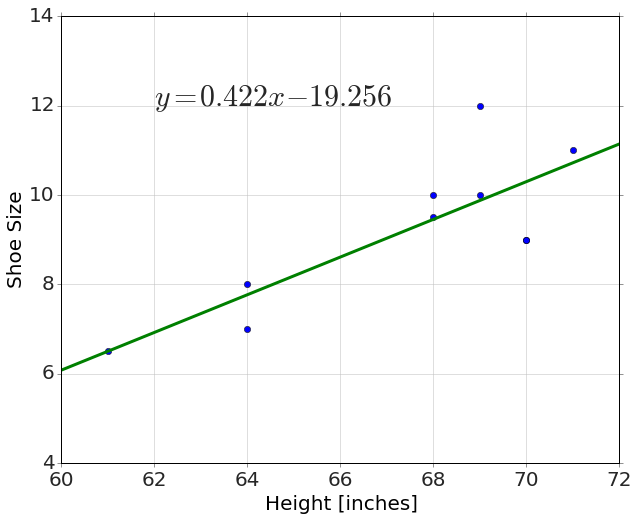
\includegraphics[width=4.5in]{Regression/Regression_fig3.png}\end{center}

\begin{lstlisting}
data=load_data('data/sat.csv')
\end{lstlisting}

\begin{lstlisting}
result=regression('total ~ expenditure',data)
\end{lstlisting}

\begin{verbatim}
<matplotlib.figure.Figure at 0x1109156d0>\end{verbatim}

\begin{center}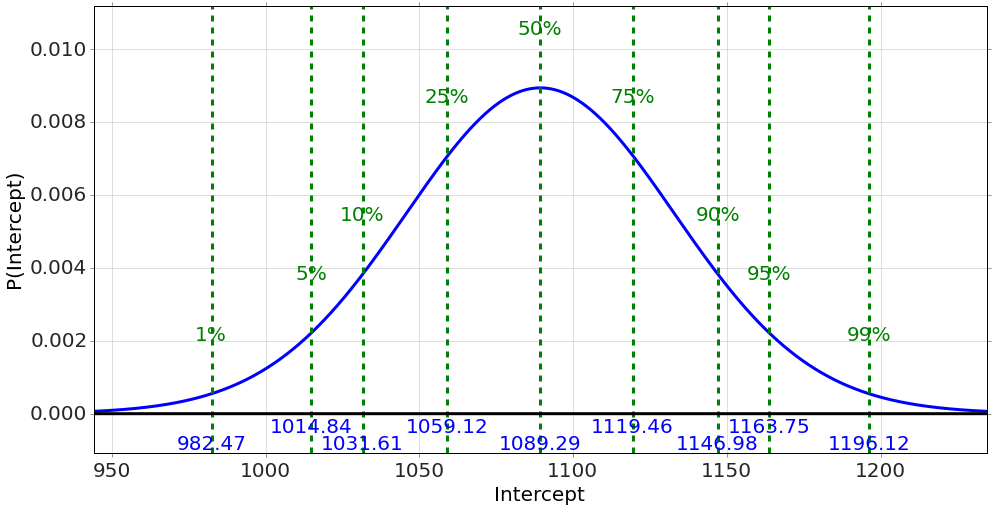
\includegraphics[width=4.5in]{Regression/Regression_fig4.png}\end{center}

\begin{verbatim}
<matplotlib.figure.Figure at 0x110953110>\end{verbatim}

\begin{center}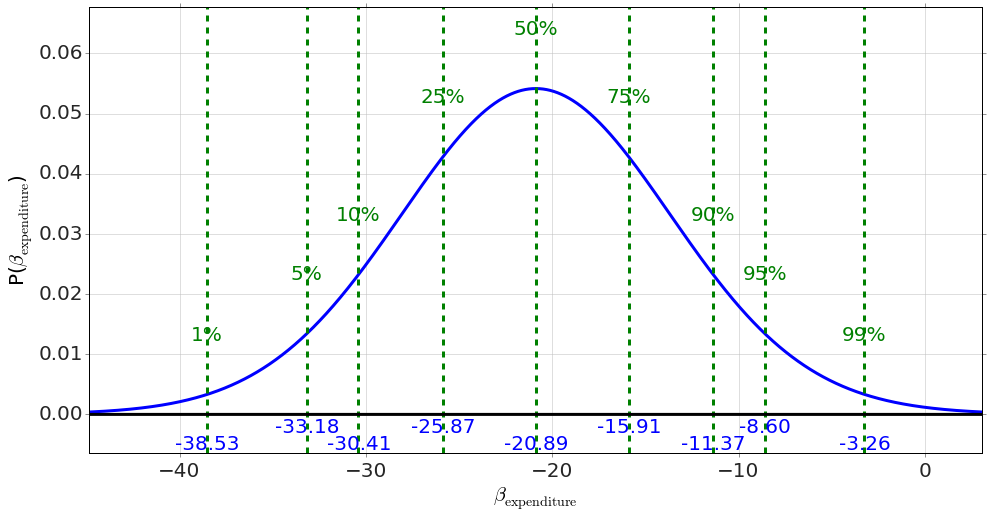
\includegraphics[width=4.5in]{Regression/Regression_fig5.png}\end{center}

\begin{lstlisting}
plot(data['expenditure'],data['total'],'o')
xlabel('Expenditure [per pupil, thousands]')
ylabel('SAT Total')
h=linspace(3,10,10)
plot(h,result['_Predict'](expenditure=h),'-')

b=result.Intercept.mean()
m=result.expenditure.mean()

if b>0:
    text(4.5,1125,'$y=%.3f x + %.3f$' % (m,b),fontsize=30)
else:
    text(4.5,1125,'$y=%.3f x %.3f$' % (m,b),fontsize=30)

\end{lstlisting}

\begin{center}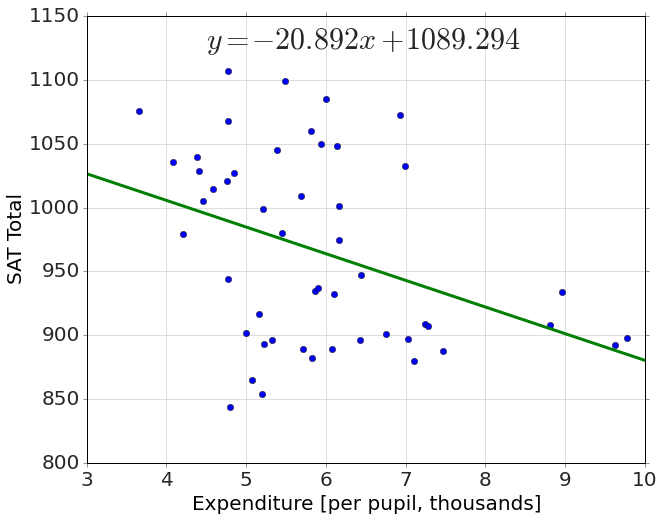
\includegraphics[width=4.5in]{Regression/Regression_fig6.png}\end{center}

\begin{lstlisting}
result=regression('percent_taking ~ expenditure',data)
\end{lstlisting}

\begin{verbatim}
<matplotlib.figure.Figure at 0x111cfff10>\end{verbatim}

\begin{center}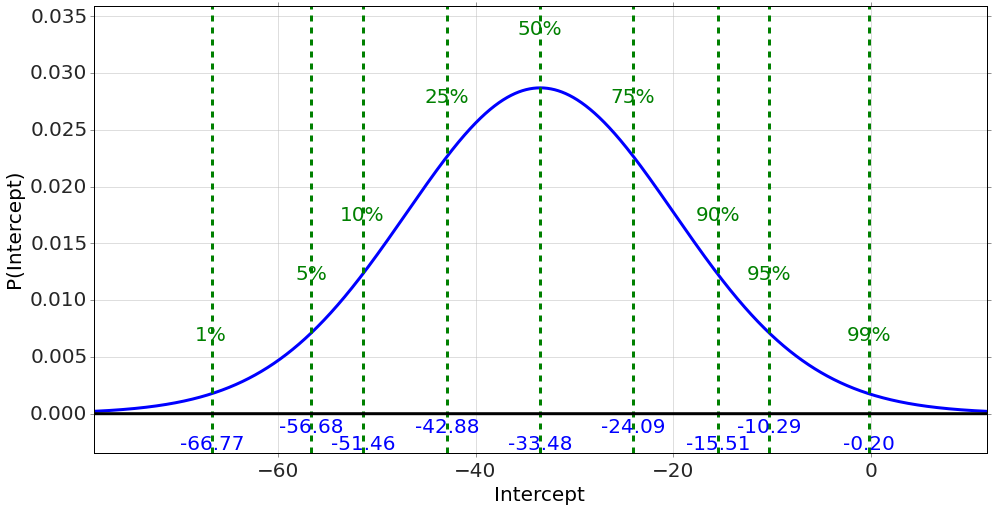
\includegraphics[width=4.5in]{Regression/Regression_fig7.png}\end{center}

\begin{verbatim}
<matplotlib.figure.Figure at 0x111867750>\end{verbatim}

\begin{center}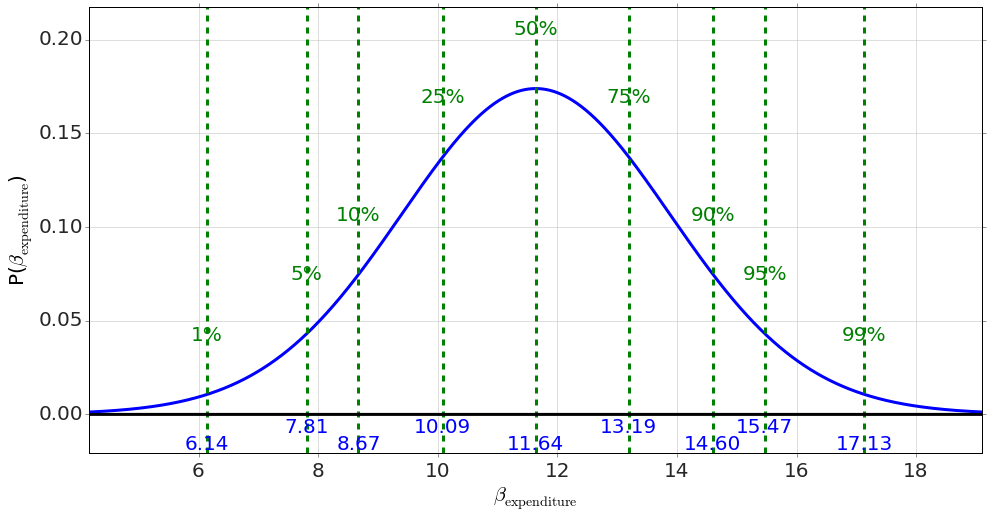
\includegraphics[width=4.5in]{Regression/Regression_fig8.png}\end{center}

\begin{lstlisting}
plot(data['expenditure'],data['percent_taking'],'o')
xlabel('Expenditure [per pupil, thousands]')
ylabel('SAT Total')
h=linspace(3,10,10)
plot(h,result['_Predict'](expenditure=h),'-')

b=result.Intercept.mean()
m=result.expenditure.mean()

if b>0:
    text(4.5,85,'$y=%.3f x + %.3f$' % (m,b),fontsize=30)
else:
    text(4.5,85,'$y=%.3f x %.3f$' % (m,b),fontsize=30)

\end{lstlisting}

\begin{center}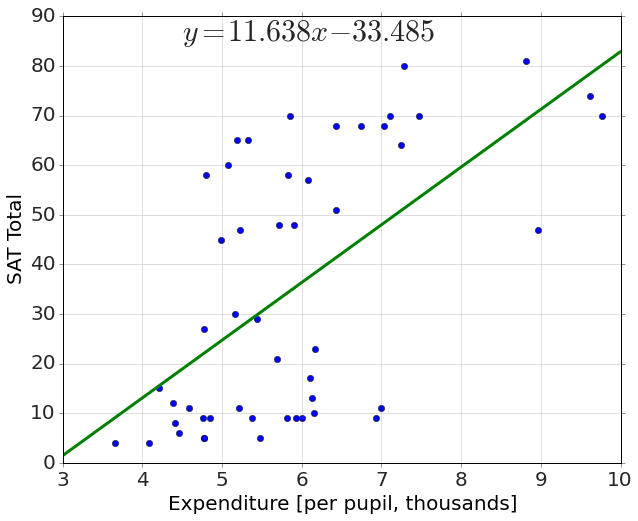
\includegraphics[width=4.5in]{Regression/Regression_fig9.png}\end{center}

\begin{lstlisting}
result=regression('total ~ expenditure + percent_taking',data)
\end{lstlisting}

\begin{verbatim}
<matplotlib.figure.Figure at 0x1107f5fd0>\end{verbatim}

\begin{center}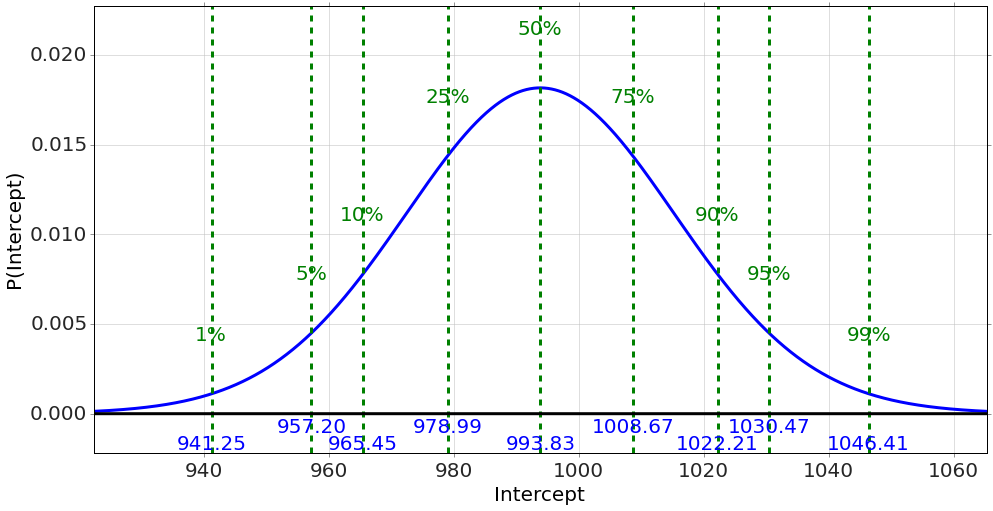
\includegraphics[width=4.5in]{Regression/Regression_fig10.png}\end{center}

\begin{verbatim}
<matplotlib.figure.Figure at 0x10d70a690>\end{verbatim}

\begin{center}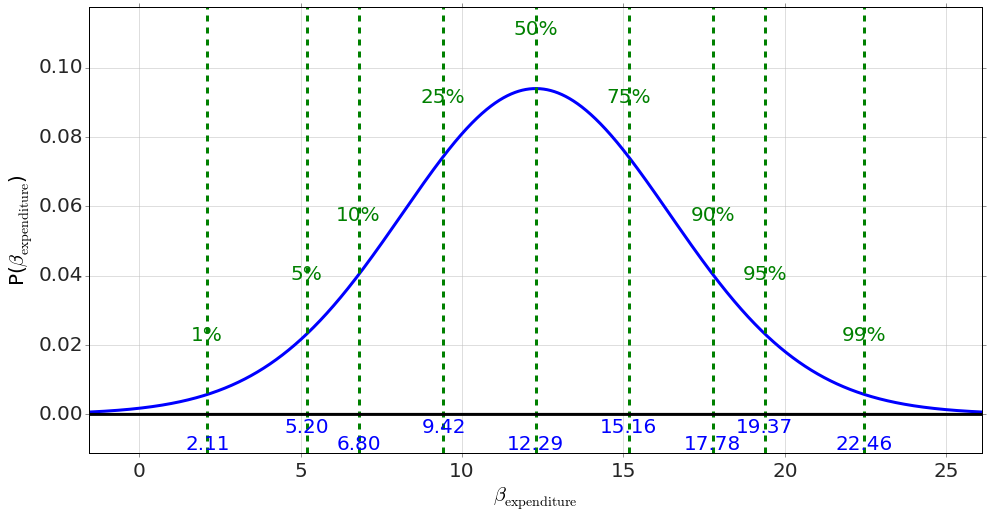
\includegraphics[width=4.5in]{Regression/Regression_fig11.png}\end{center}

\begin{verbatim}
<matplotlib.figure.Figure at 0x110fbcf90>\end{verbatim}

\begin{center}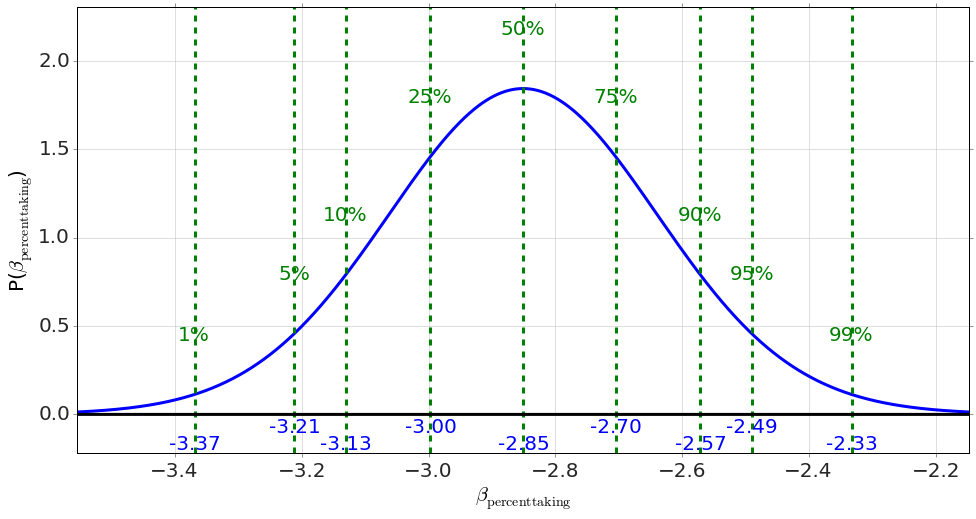
\includegraphics[width=4.5in]{Regression/Regression_fig12.png}\end{center}

\begin{lstlisting}

\end{lstlisting}


\end{fullwidth}